% 8 variables in here:
% u_1 = 0.0, h_1 = 10.0, U_1 = 0.0, H_1 = 10.0, u_2 = 0.0, h_2 = 10.0, U_2 = 0.0, H_2 = 10.0
\begin{figure}[h!t]
\centering
  % \subfigure[Height error] {
  %   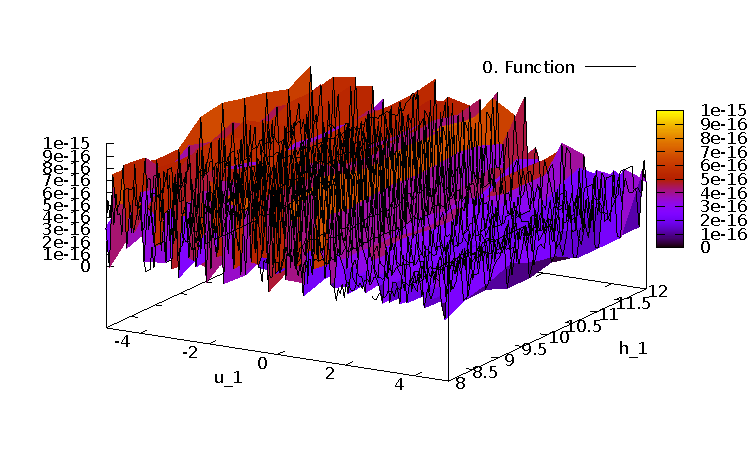
\includegraphics[scale=\zoomfactor]{{{2_points_def_luecke/x_y_0.0_10.0_0.0_10.0_0.0_10.0f0}}}
  % }
  % \subfigure[Impulse error] {
    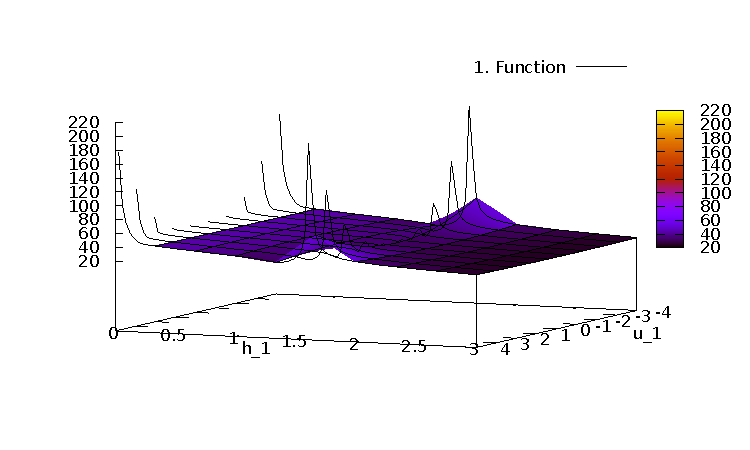
\includegraphics[scale=\zoomfactor]{{{2_points_def_luecke/x_y_0.0_10.0_0.0_10.0_0.0_10.0f1}}}
  % }
\caption{Plotting the impulse error depending on $p_1$ for a wider range. All other points are $(10,0)$.}
\label{fig:two-points-p1-wider-range}
\end{figure}

%%% Local Variables:
%%% TeX-master: "../results.tex"
%%% End:

%%% Local Variables:
%%% TeX-master: "../results.tex"
%%% End:
